
\makequotation{It is practically impossible to teach good programming to
  students that have had a prior exposure to BASIC: as potential
  programmers they are mentally mutilated beyond hope of
  regeneration.}{Edsger W. Dijkstra, Turing Award winner}

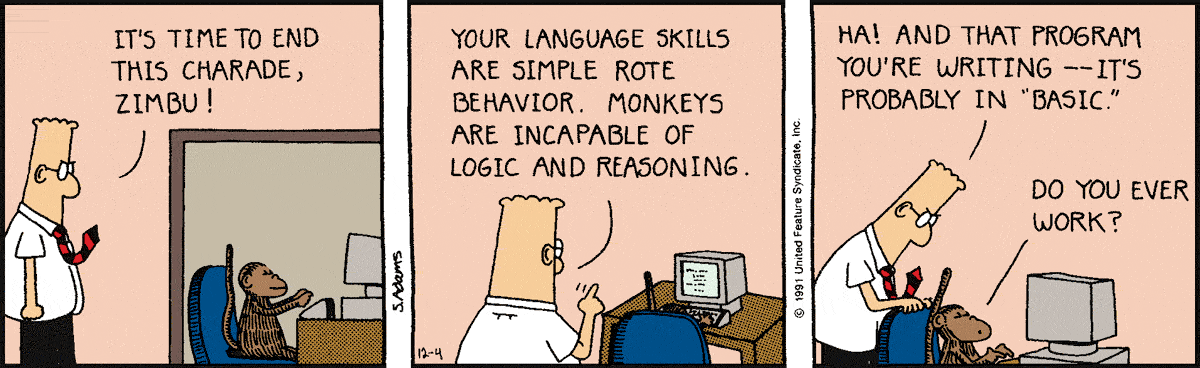
\includegraphics[width=\textwidth]{figs/dilbert-1991-12-04.png}

%% \makequotation{\ldots the teaching of BASIC should be rated as a
%%   criminal offence: it mutilates the mind beyond recovery.}{Edsger
%%   W. Dijkstra, Turing Award winner}

%% \makequotation{I think it's fair to say that more persons in the world know how to
%% write simple programs in BASIC than in any other language. It is true
%% that most of them are probably still unable to vote or buy a drink.  And
%% if FORTRAN is the lingua franca, then certainly it must be true that
%% BASIC is the lingua playpen.}{Thomas E. Kurtz, co-creator of BASIC, in
%%   1981~\cite{hopl}} 

Much has been written over the decades about the democratization of
computers thanks to Moore's Law, but what has been overlooked is that up
until the consumer Internet appeared in around 1995, BASIC was present
at every milestone, and played a pivotal role in empowering generations
of programmers.
Yet BASIC is probably one of the most maligned programming languages
to achieve widespread use.

In \emph{Back to BASIC}~\cite{backtobasic}, the language's co-creators
object that the criticisms leveled at the 
BASIC dialects that proliferated after BASIC became the
\emph{lingua franca} of PCs did not apply to the original language
they had created and to its designated descendants.
This defense seems doubtful, since the original language did include
\T{GO~TO}, which Dijkstra famously railed
against~\cite{goto_considered_harmful}.

In the 2006 Salon article~\cite{why_johnny_cant_code},
science fiction author David Brin laments that for all its flaws, 
despite its small view of the world (or perhaps because of it), BASIC
was sufficiently nonthreatening to introduce an entire generation of
newbies to the joy of programming---exactly the goals of its
creators---whereas today's more expressive languages for higher-powered
platforms may scare beginners away.
Many angry responses to Brin's article pointed out that BASIC
instills habits contrary to modern object-oriented programming practices (true),
that powerful scripting languages like Perl and Python have filled BASIC's
niche (true), and so on.  

In both pieces of writing, the criticisms as well as the responses miss
the point.
Perl and Python are indeed better designed than BASIC, but they are
targeted at professional programmers, not beginners, and they reflect
two decades of thinking and experience focused on a professional
audience, not a student audience.
These languages can be intimidatingly powerful for beginners (though
Python can be suitably simplified by simply not using some of its
advanced
features).\footnote{\href{http://quitebasic.com}{QuiteBASIC.com}, an
in-browser BASIC environment developed in response to Brin's article, is
a good proxy for the ``old school BASIC'' Brin praises.}

The real goal of BASIC was to expose as many non-programmers as possible
to programming---and this it accomplished beyond its creators' wildest
dreams, if not in the precise manner they had envisioned.
With the help of a wide cast of characters who wittingly or unwittingly
played key roles in BASIC's dissemination---Bob Albrecht, David Ahl,
Paul Allen, Dennis Allison, Bill Gates, Chuck Peddle, Ed Roberts,
Li-Chen Wang, Steve Wozniak, and the companies and institutions where
they worked---BASIC introduced an entire generation of programmers to
programming.
If it inculcated ``bad'' habits in us that structured languages tried to
break, it also taught us computational thinking.

It's time the true story of BASIC's influence was told.
